\subsection{Tecnologías utilizadas para la interfaz gráfica}
\label{subsec:gui-tecnologias}

La interfaz de escritorio utiliza JavaFX 17.0.2 con FXML y CSS. JavaFX aporta la ventana, escenas, controles, eventos y tablas; FXML declara la jerarquía visual y enlaza nodos con clases controladoras; CSS aplica los estilos compartidos. El plugin Maven de JavaFX configura \texttt{com.overbyte.Main} como clase de inicio para la ejecución mediante Maven. Existe además otro \texttt{Main} en el paquete por defecto con un menú de consola y una opción para iniciar la GUI; no es el punto de entrada configurado en el plugin JavaFX.

\subsubsection{Tecnología de interfaz gráfica}

El método de inicio de la aplicación prepara la ventana y el navegador, y carga la vista de acceso mediante \texttt{FXMLLoader}. El cargador construye los controles, inyecta los campos anotados y ejecuta la inicialización de cada controlador. La aplicación carga hojas de estilo y cambia las vistas de acuerdo con el rol. Las pantallas incluyen formularios, botones, campos, tablas/listas, navegación lateral y cuadros de diálogo.

El tamaño inicial de la ventana y las dimensiones mínimas se definen en la aplicación; no debe interpretarse que la ventana sea invariable si el usuario puede redimensionarla. La GUI emplea estilos consistentes y una paleta visual predominante en violeta, como se aprecia en las capturas. No se halló un framework adicional de componentes ni una herramienta automática de interacción gráfica dentro de las dependencias de Maven.

\subsubsection{Diseño de interfaces y capturas disponibles}

Las imágenes siguientes son capturas que ya estaban en el repositorio. Se incorporan sin alteración y se describen como estados visuales puntuales. Una captura no prueba que una acción representada por un botón se haya ejecutado correctamente. Para la captura del carrito existe además una diferencia con el FXML actual: la vista vigente solicita nombre, CI y teléfono, mientras que la imagen muestra solo el campo de nombre; no se puede determinar la fecha exacta de la imagen, por lo que no se le asigna una versión concreta.

\paragraph{Captura 1. Inicio de sesión.}
La pantalla muestra el nombre del sistema, el campo de usuario, selección del rol (administrador, cajero o almacén), contraseña y botón de inicio de sesión. Técnicamente corresponde al acceso previo a la navegación por rol. La imagen demuestra la composición visual del formulario, no el resultado de una autenticación real.

\begin{figure}[H]
\centering
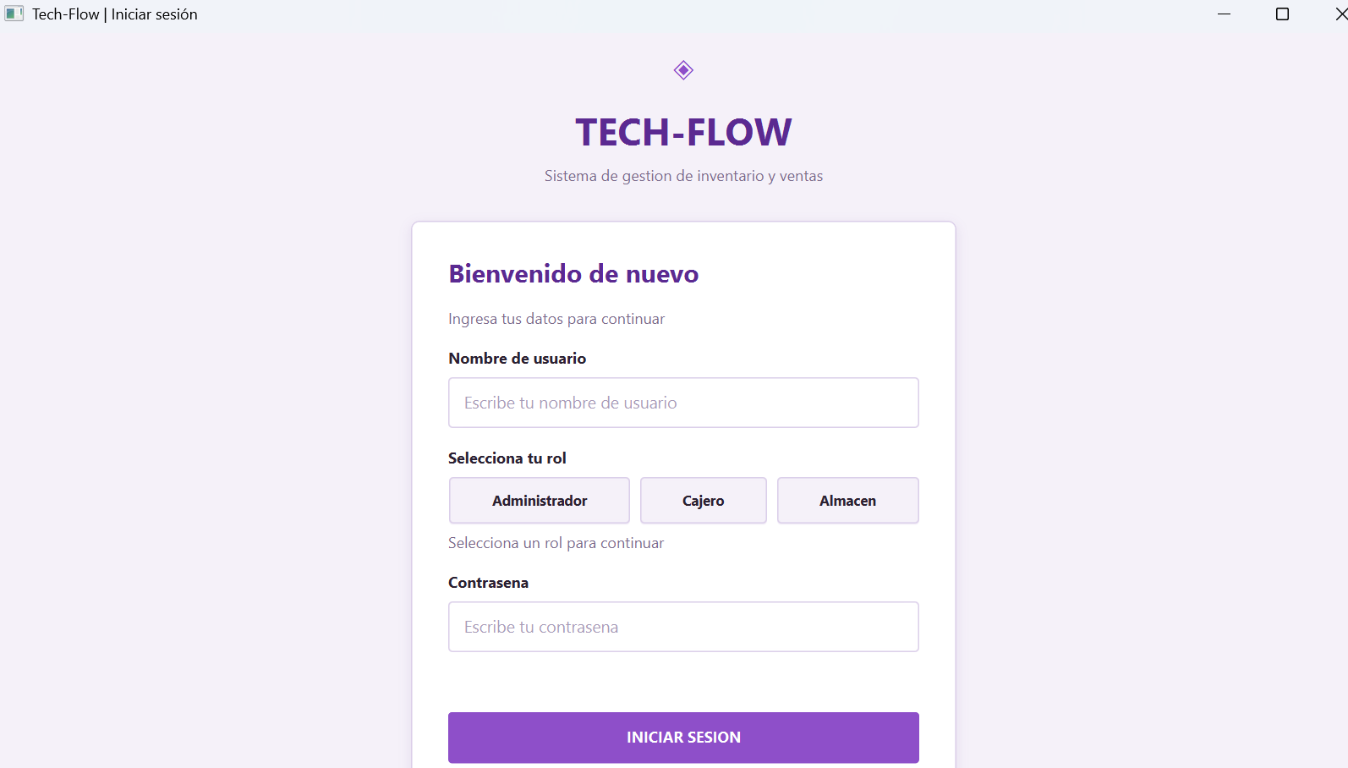
\includegraphics[width=0.93\textwidth,height=0.40\textheight,keepaspectratio]{../capturas/01-login.png}
\caption{Captura 1. Pantalla de inicio de sesión y selección de rol.}
\label{fig:captura-login}
\end{figure}

\paragraph{Captura 2. Administración y apertura de caja.}
La imagen presenta la ventana de administración en la sección de ventas, oscurecida por un diálogo que pregunta si se desea abrir la caja. Se observan los controles \textit{Abrir caja} y \textit{Ahora no}. El diálogo explica que la operación de ventas requiere habilitar caja. El estado visible es \textit{CERRADA}; no se presenta la captura como prueba de que el botón se haya pulsado ni de que la caja se haya abierto.

\begin{figure}[H]
\centering
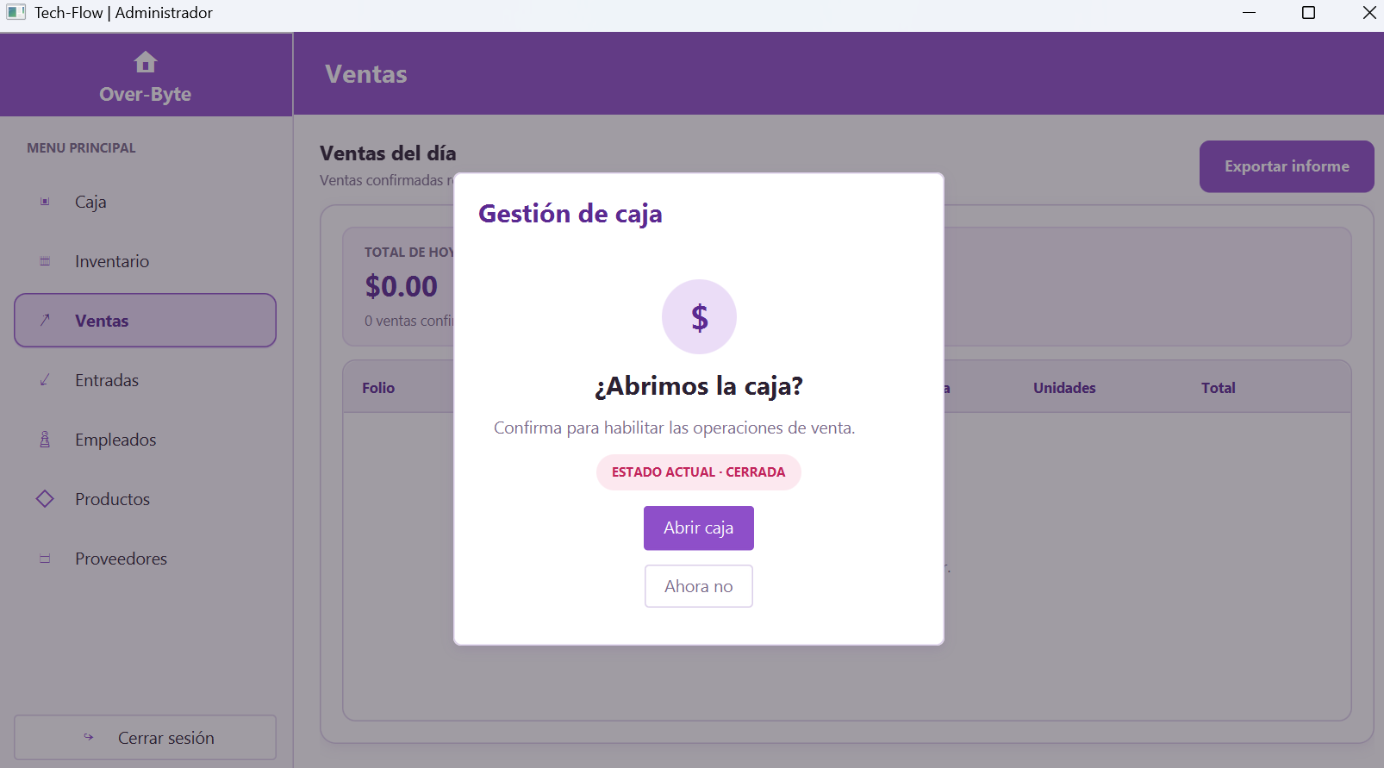
\includegraphics[width=0.93\textwidth,height=0.40\textheight,keepaspectratio]{../capturas/02-admin-caja.png}
\caption{Captura 2. Vista administrativa de ventas con el diálogo de caja cerrada.}
\label{fig:captura-caja}
\end{figure}

\paragraph{Captura 3. Consulta de ventas del día.}
La interfaz muestra el total de hoy como \$0.00 y cero ventas confirmadas, junto con una tabla vacía y el botón \textit{Exportar informe}. Es un estado puntual de la captura: no demuestra que el sistema nunca registre ventas ni que el informe se haya exportado. Técnicamente representa una consulta de ventas confirmadas del día.

\begin{figure}[H]
\centering
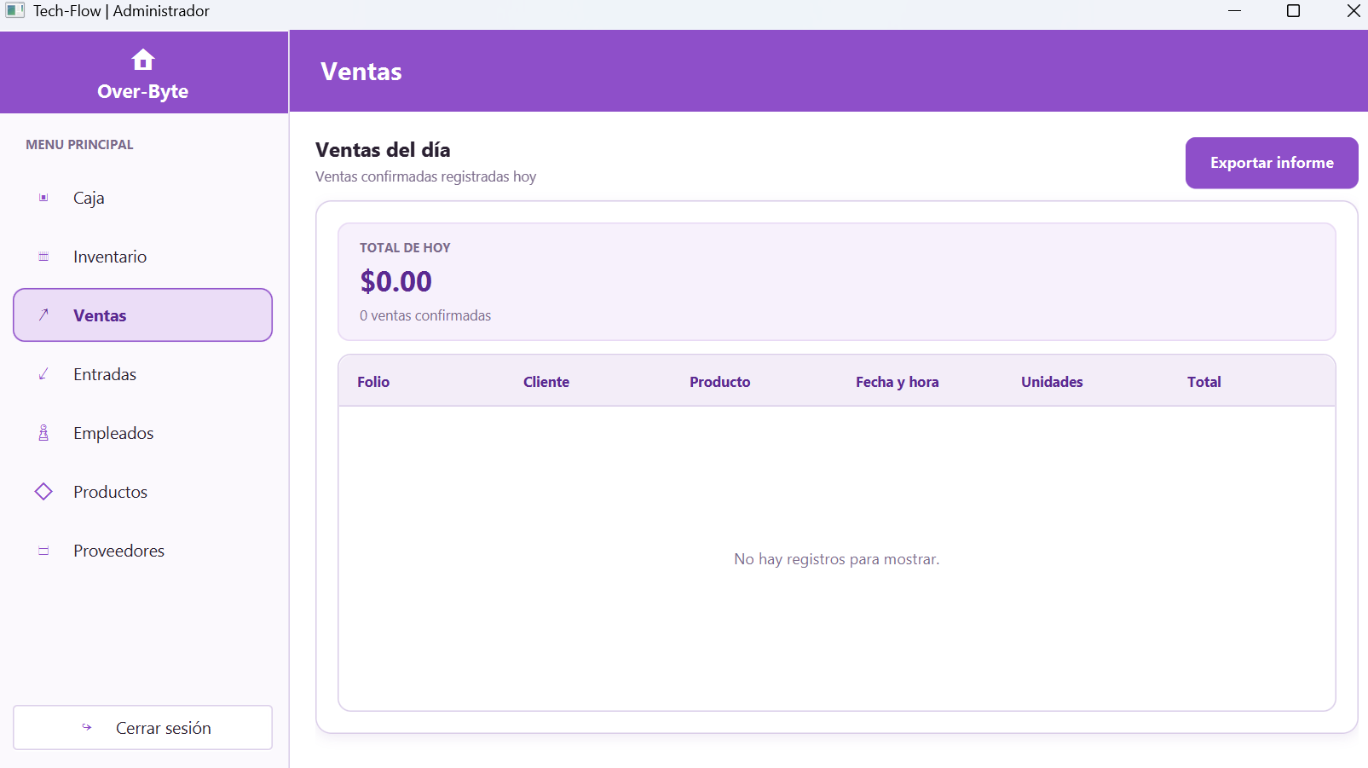
\includegraphics[width=0.93\textwidth,height=0.40\textheight,keepaspectratio]{../capturas/03-admin-ventas.png}
\caption{Captura 3. Sección administrativa de ventas del día, sin registros visibles en ese instante.}
\label{fig:captura-ventas}
\end{figure}

\paragraph{Captura 4. Carrito del vendedor.}
Se observan un artículo seleccionado, cantidad cuatro, subtotal y total, además de acciones para confirmar venta, crear proforma, vaciar el carrito, anular y consultar garantía o importar una orden CSV. La imagen permite explicar las operaciones disponibles en la vista. No prueba la finalización de ninguna de ellas. Como se indicó, el formulario visible en la imagen no muestra CI ni teléfono; el FXML actual los exige junto con el nombre del cliente.

\begin{figure}[H]
\centering
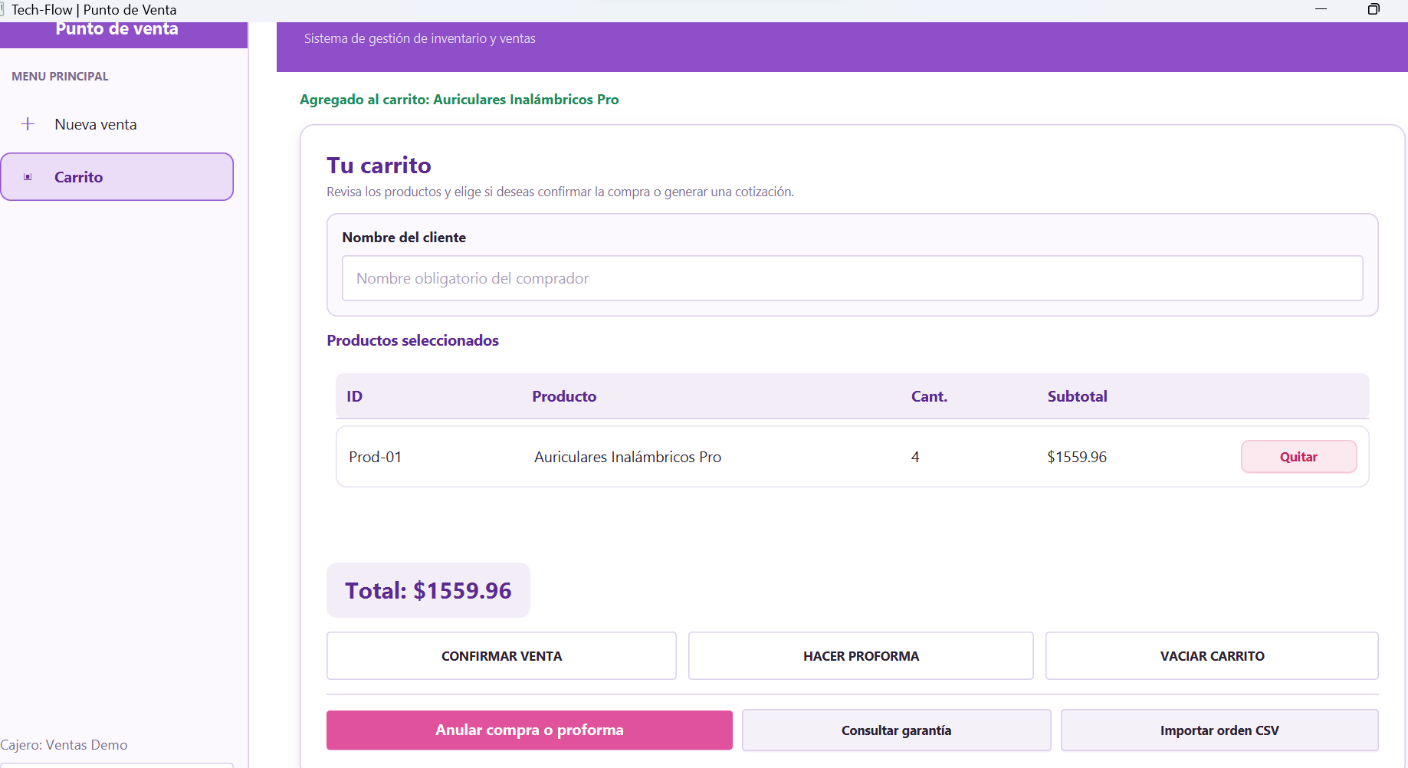
\includegraphics[width=0.93\textwidth,height=0.40\textheight,keepaspectratio]{../capturas/04-cajero-carrito.png}
\caption{Captura 4. Carrito del vendedor con un producto seleccionado y acciones de venta/proforma.}
\label{fig:captura-carrito}
\end{figure}

\paragraph{Captura 5. Consulta del inventario de almacén.}
La vista presenta una tabla con identificador, nombre, marca, categoría, precio de compra, precio de venta y existencias, junto con las acciones para registrar un producto o navegar a entradas. Es una representación de la consulta de inventario del almacenero. Los valores visibles pertenecen al estado capturado y no son métricas permanentes del sistema.

\begin{figure}[H]
\centering
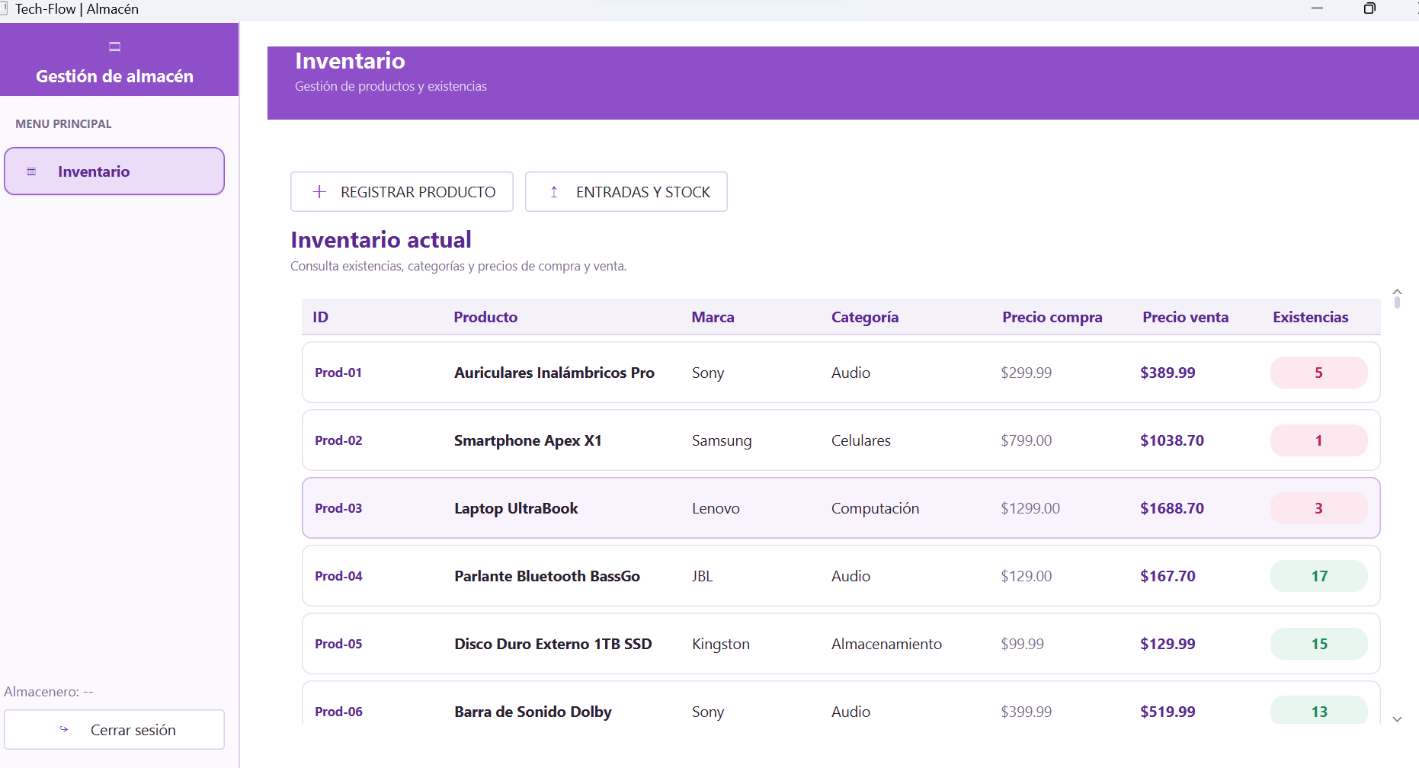
\includegraphics[width=0.93\textwidth,height=0.40\textheight,keepaspectratio]{../capturas/05-almacen-inventario.png}
\caption{Captura 5. Inventario actual en la interfaz de almacén.}
\label{fig:captura-inventario}
\end{figure}

\paragraph{Captura 6. Selección de productos para una entrada.}
La pantalla permite buscar productos y presenta la lista de productos disponibles junto a un panel de entradas seleccionadas. En la parte inferior se aprecian las acciones para importar entradas CSV, registrar entradas y cerrar. La interfaz ilustra la preparación de una entrada; no demuestra que se haya importado un archivo o actualizado el stock.

\begin{figure}[H]
\centering
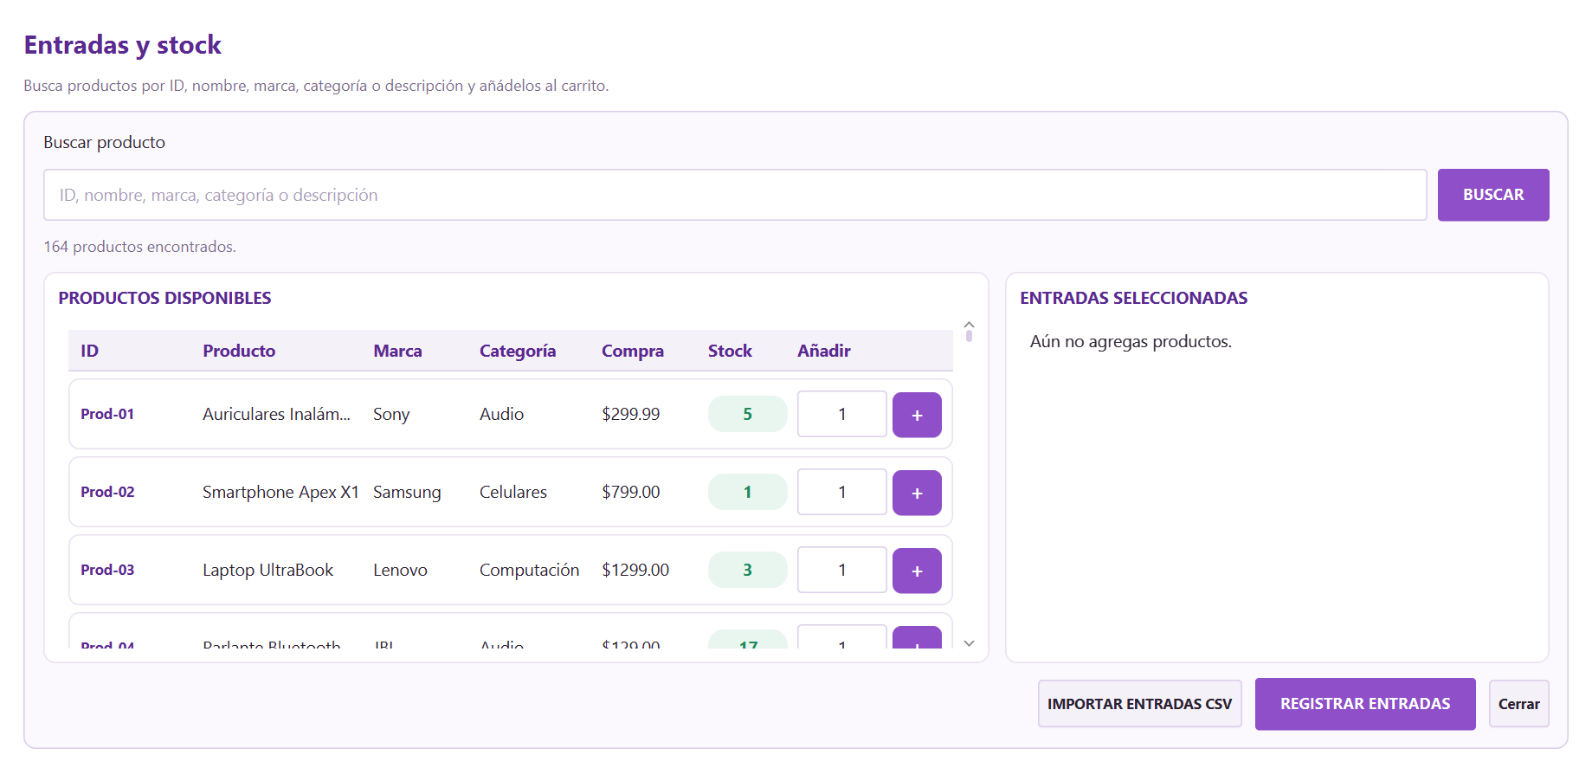
\includegraphics[width=0.93\textwidth,height=0.40\textheight,keepaspectratio]{../capturas/06-almacen-entradas.png}
\caption{Captura 6. Interfaz de selección y registro de entradas de almacén.}
\label{fig:captura-entradas}
\end{figure}

\subsubsection{Conexión de la GUI con el sistema}

Las acciones de botones y campos están conectadas a controladores declarados desde FXML. El controlador obtiene los datos de los componentes, aplica controles de interfaz cuando corresponde, invoca servicios o clases de dominio y actualiza tablas, mensajes o diálogos. Por ejemplo, la pantalla de vendedor reúne datos del carrito y del comprador; la lógica de dominio distingue crear proforma de confirmar la venta; la respuesta se utiliza para refrescar el estado visual y comunicar el resultado.

En el acceso, \texttt{LoginController} entrega las credenciales y el rol elegido a \texttt{Verificador}; ante un resultado nulo muestra el mensaje de rechazo y, ante un empleado válido, deriva a la vista correspondiente:

\begin{lstlisting}[language=Java,caption={Fragmento real de coordinación de autenticación en LoginController.},label={lst:login-controller},literate={ñ}{{\~n}}1]
Empleado empleado = verificador.iniciarSesion(
    nombre,
    contrasena,
    rolSeleccionado
);
if (empleado == null) {
    mensaje.setText("Nombre, contraseña o rol incorrectos.");
    campoContrasena.clear();
    campoContrasena.requestFocus();
    return;
}
abrirVistaSegunRol(empleado);
\end{lstlisting}

En almacén, la interfaz permite seleccionar productos/cantidades y registrar o importar entradas; la clase de dominio valida proveedor, producto, precio y cantidad antes de persistir. En administración, el controlador coordina caja, consultas y exportaciones. Como algunos controladores leen CSV directamente, no todas las consultas siguen la ruta controlador--modelo--servicio. El comportamiento de acceso inválido depende de validaciones y mensajes específicos; no se encontró evidencia de una política uniforme de errores de interfaz para todos los formularios.

\subsection{Pruebas funcionales a nivel de usuario basadas en escenarios}
\label{subsec:escenarios}

Los siguientes casos de uso son escenarios de validación manual derivados de funcionalidades verificadas en el código. Los pasos describen qué debería comprobar una prueba de usuario; no afirman que se haya ejecutado una sesión gráfica de extremo a extremo durante esta revisión. Las pruebas JUnit de dominio y CSV sí cubren reglas relacionadas, pero no equivalen a pulsar los controles y observar la respuesta completa de la GUI.

\begin{longtable}{|p{0.85cm}|p{2.1cm}|p{3.3cm}|p{4.0cm}|p{2.4cm}|}
\caption{Escenarios funcionales de usuario propuestos a partir del sistema implementado.}
\label{tab:escenarios-usuario}\\
\hline
\textbf{ID} & \textbf{Escenario} & \textbf{Precondiciones / datos} & \textbf{Pasos y respuesta esperada} & \textbf{Estado de GUI}\\
\hline
\endfirsthead
\hline
\textbf{ID} & \textbf{Escenario} & \textbf{Precondiciones / datos} & \textbf{Pasos y respuesta esperada} & \textbf{Estado de GUI}\\
\hline
\endhead
EU-01 & Acceso por rol & Empleado existente y credenciales válidas para un rol. & Ingresar credenciales, elegir rol e iniciar sesión; se espera abrir la vista correspondiente. & No ejecutado en esta revisión.\\
\hline
EU-02 & Crear proforma & Caja/datos de prueba y producto existente con stock. & Seleccionar producto y cantidad, completar datos del cliente y elegir proforma; se espera mostrar la operación sin descontar ni reservar stock. & No ejecutado en GUI; regla cubierta por prueba de dominio.\\
\hline
EU-03 & Confirmar venta & Caja abierta y stock suficiente; cliente y carrito válidos. & Confirmar la venta; se espera registrar la operación, actualizar stock y conservar cliente/garantías. & No ejecutado en GUI; reglas parciales cubiertas por JUnit.\\
\hline
EU-04 & Rechazar venta sin caja o sin stock & Caja cerrada o cantidad mayor al stock. & Intentar confirmar; se espera impedir el registro y comunicar que la precondición no se cumple. & No ejecutado en GUI; condiciones probadas en dominio.\\
\hline
EU-05 & Registrar entrada importada & CSV con encabezados/campos requeridos y proveedor existente. & Importar el archivo y confirmar la operación; se espera actualizar o crear productos y registrar las entradas. & No ejecutado en GUI; importación probada en dominio.\\
\hline
EU-06 & Rechazar entrada inválida & Proveedor inexistente, cantidad negativa o fila incompleta. & Seleccionar/importar datos inválidos; se espera rechazar la operación sin aceptar el cambio de stock. & No ejecutado en GUI; casos inválidos probados en dominio.\\
\hline
\end{longtable}

Los casos EU-02 a EU-06 no deben considerarse una prueba visual aprobada solo porque existan pruebas unitarias relacionadas. La verificación de usuario deberá ejecutarse en una instalación aislada con datos de prueba, comprobar el mensaje y los controles, y confirmar el contenido final de los CSV. La captura del carrito tampoco valida el formulario actual completo, dado que no muestra dos campos presentes en el FXML revisado.

\subsection{Resultados de la validación y evidencias disponibles}

La evidencia disponible permite distinguir tres niveles. Primero, el código y las pruebas JUnit comprueban reglas de dominio y persistencia bajo condiciones controladas. Segundo, las capturas muestran pantallas representadas y ciertos estados visuales concretos. Tercero, no hay en el repositorio una suite automatizada de interacción gráfica que valide de extremo a extremo los formularios, la navegación y la actualización visual. Por eso, los escenarios de usuario quedan especificados, pero su estado de ejecución en GUI es \textit{no ejecutado en esta revisión}.

\begin{longtable}{|p{3.5cm}|p{4.6cm}|p{5.1cm}|}
\caption{Alcance de las evidencias disponibles para la FASE 3.}
\label{tab:evidencia-fase3}\\
\hline
\textbf{Evidencia} & \textbf{Qué permite sostener} & \textbf{Qué no permite concluir}\\
\hline
\endfirsthead
\hline
\textbf{Evidencia} & \textbf{Qué permite sostener} & \textbf{Qué no permite concluir}\\
\hline
\endhead
Pruebas JUnit de dominio y servicios & Reglas puntuales de venta, stock, importación, validación y filas CSV bajo los casos incluidos. & Que todas las pantallas, botones y secuencias de navegación funcionen de extremo a extremo.\\
\hline
Capturas 1--6 & Composición visual y estado visible de acceso, administración/caja, ventas, carrito e inventario/entradas. & Que el contenido sea el estado universal del sistema, que los controles hayan sido activados o que las operaciones se hayan completado.\\
\hline
FXML y controladores actuales & Estructura declarada de vistas, eventos y coordinación con operaciones Java. & Que no existan errores de ejecución en toda interacción posible; la revisión no ejecutó una campaña manual completa de GUI.\\
\hline
Registro histórico de cambios & Indica que se documentó una comprobación de carga de vistas JavaFX en una etapa anterior. & No permite reproducir ni atribuir un resultado actual a una clase de prueba fuente que no se encontró.\\
\hline
\end{longtable}
